% !TeX program = xelatex
% !TeX encoding = UTF-8
% !TeX TXS-program:bibliography = txs:///bibtex
\documentclass[11pt]{article}

% ============================================================
% Build order (important):
%   1) XeLaTeX qsr_rag_acl_chinese_review.tex
%   2) BibTeX  qsr_rag_acl_chinese_review
%   3) XeLaTeX qsr_rag_acl_chinese_review.tex
%   4) XeLaTeX qsr_rag_acl_chinese_review.tex
%
% Files that must be in the same project directory:
%   qsr_rag_acl_chinese_review.tex
%   qsr_rag.bib
%   acl.sty
%   acl_natbib.bst
%   figures/figure1.pdf
%   figures/figure2.pdf
%   figures/figure3_accuracy_token.pdf
% ============================================================

% ACL/COLING 风格匿名评审格式；若用于 camera-ready，可按要求移除 [review]。
% 正文目标：在官方 ACL 模板下，参考文献之前约 7 页。
% 完整统计表、提示词细节、资源消耗表和定性轨迹均放在附录中。
\usepackage[review]{acl}
\usepackage{times}
\usepackage{latexsym}
\usepackage{graphicx}
\usepackage{amsmath}
\usepackage{amssymb}
\usepackage{booktabs}
\usepackage{array}
\usepackage{tabularx}
\usepackage{makecell}
\usepackage{microtype}
\usepackage[UTF8]{ctex}

\setlength\titlebox{6cm}
\renewcommand{\arraystretch}{1.08}
% Keep review line numbers inside the narrow inter-column gutter.
\setlength{\linenumbersep}{4pt}
\raggedbottom
\emergencystretch=1.5em

\title{QSR-RAG：面向多跳检索增强生成的\\
	基于证据的问题状态重写}

\author{匿名作者}

\begin{document}
	\maketitle

	\begin{abstract}
		在多跳检索增强生成（RAG）中，随着中间证据不断获得，系统的信息需求也会随之演化。现有迭代式 RAG 方法主要关注生成下一条检索查询、子问题或推理轨迹，而对如何将“当前问题本身”作为一个跨轮次持续存在的状态关注较少。我们提出 QSR-RAG，将固定不变的目标问题（Target Question）与持续演化的推理问题（Reasoning Question）区分开来。在每一轮中，系统检索并验证局部答案，将被接受的中间事实存入已验证解答记忆（Verified Resolution Memory），再通过替换（Substitution）或增强（Augmentation）来更新推理问题，使后续检索从一个已经反映此前推理进展的任务表述出发。我们在 HotpotQA、2WikiMultiHopQA 和 MuSiQue 上，使用 GPT-4o-mini 与 Qwen3-8B 对 QSR-RAG 进行评测。在共享检索后端的条件下，QSR-RAG 在全部六种设置中都取得了最高的 EM/F1。与“仅记忆（Memory-only）”对照设置相比——该设置保留已验证记忆和动态局部问题生成，但不更新问题状态——QSR-RAG 的平均 EM 和 F1 分别提升 2.44 和 2.41 个百分点。结果表明，即使外部记忆已经能够影响后续查询，持续更新当前问题本身仍然能够带来额外收益。
	\end{abstract}

	\section{引言}

	检索增强生成（RAG）将语言模型的参数化知识与外部证据相结合，以提高知识密集型任务中的事实可靠性 \citep{guu2020realm,lewis2020rag,izacard2021fid,gao2023ragsurvey}。在标准的“检索后阅读（Retrieve-then-Read）”流程中，原始问题通常被直接同时用于检索和回答。然而，多跳问题有所不同：其中的实体、属性和关系彼此依赖，后续跳的信息往往必须等到前面的实体或关系被解析后才能被直接检索。因此，一个有效的多跳 RAG 系统仅仅覆盖足够多的证据还不够，它还需要表示哪些内容已经被解析，以及在这些解析结果基础上，剩余任务应该如何重新表述。

	现有方法已经会利用中间结果来生成后续问题、扩展推理轨迹或重写后续查询 \citep{press2023selfask,trivedi2023ircot,shao2023iterretgen,zhu2025chainrag,ji2025dec,kim2025unirag}。我们关注的问题更具体：\emph{如果系统已经能够把中间事实存入记忆，并利用这些事实动态生成下一条局部查询，那么持续更新一个完整的自然语言问题是否仍然有价值？} 这一区分对应于两个不同问题：“下一步应该检索什么？”以及“经过前几轮之后，当前任务究竟是什么？”QSR-RAG 将后者显式建模为一个持久状态。

	QSR-RAG 维护四类信息。目标问题 $Q^{(0)}$ 始终保持不变，用于锚定原始任务及其答案空间。推理问题 $Q^{(t)}$ 会随着已验证的中间事实而更新，用来表示任务在当前时刻的表述。已验证解答记忆 $M^{(t)}$ 存储被接受的中间解答。相比之下，局部问题 $q^{(t)}$ 只是一轮中的检索动作。记忆记录“已经知道什么”，而推理问题记录“这些事实如何改变当前剩余任务的表述”。局部问题是临时的，而推理问题会持续进入下一轮。

	以“Tokarev 任教的那所大学是什么时候建立的？”为例。系统可以先询问“Sergei Tokarev 在哪所大学任教？”如果检索到的证据支持 \emph{Moscow State University}，该事实就会被加入记忆，推理问题则可以更新为“莫斯科国立大学是什么时候建立的？”我们将这种对隐藏实体进行解析的操作称为 \textbf{实体绑定替换（Entity-Binding Substitution）}，下文简称 \textbf{替换（Substitution）}。但对于比较、选择或布尔问题，直接替换可能改变候选项或最终答案空间。此时，QSR-RAG 使用 \textbf{上下文注入增强（Context-Injection Augmentation）}，下文简称 \textbf{增强（Augmentation）}：保留原问题结构，同时把已验证事实作为前提加入其中。两种操作都会更新持久的推理问题，而局部问题仍然只是一次临时检索动作。

	持久状态也会带来新的失败模式：一旦错误的中间事实或不安全的重写被带入后续轮次，后续检索就可能从错误状态继续进行。因此，QSR-RAG 在状态更新之前加入答案适配器（Answer Adapter）。适配器检查两个方面：局部阅读器（Local Reader）的答案是否确实填补了当前解答目标（Resolution Target），以及检索证据是否直接支持该关系。只有通过检查的结果才能进入已验证解答记忆，并具备更新状态的资格。该检查关注的是“关系是否得到支持”，而不是简单的词面匹配；仅仅在证据中看到了答案字符串并不足够。

	我们在 HotpotQA、2WikiMultiHopQA 和 MuSiQue 上使用 GPT-4o-mini 与 Qwen3-8B 评估 QSR-RAG。除完整系统比较外，我们还引入了“仅记忆（Memory-only）”对照设置。该设置仍会利用累计记忆和局部问题历史动态生成新的局部问题，但保持推理问题不变。由此，我们可以直接比较“记忆 + 动态查询”和“记忆 + 动态查询 + 持久的问题状态更新”。完整 QSR-RAG 在三个数据集上的点估计都更高，其中 2WikiMultiHopQA 的差异以及跨数据集聚合分析都获得了统计支持。

	我们的主要贡献如下：
	\begin{enumerate}
		\item 我们区分了临时的局部问题与跨轮次持续存在的推理问题，并研究：当记忆已经能够保留并复用中间事实时，进一步更新当前完整问题是否仍能带来收益。
		\item 我们提出 QSR-RAG：先将经过验证的局部解答存入记忆，再通过替换或增强把这些解答写入推理问题，使后续检索从已经反映已验证推理进展的任务表述开始。
		\item 我们在三个多跳问答数据集和两个主干模型上评估该框架，并进行了仅记忆、单一更新策略和答案适配器等消融实验。问题状态更新在三个数据集上的 F1 点估计均为正，其中 2WikiMultiHopQA 上的增益在 Holm 校正后仍具有统计显著性。
	\end{enumerate}

	\section{相关工作}

	\subsection{迭代检索与查询重写}
	RAG 与开放域问答研究已经发展出稀疏检索、稠密检索、段落融合、对比式稠密检索和后交互（late interaction）等方法 \citep{guu2020realm,lewis2020rag,karpukhin2020dpr,izacard2021fid,izacard2022contriever,khattab2020colbert,izacard2023atlas}。多跳场景进一步提出了一个要求：中间结果必须能够影响后续搜索。早期的迭代式检索器--阅读器系统以及压缩式多跳检索已经遵循这一思想 \citep{das2019multistep,khattab2021baleen,yang2018hotpotqa,ho2020twowiki,trivedi2022musique}。IRCoT 和 Iter-RetGen 进一步把推理或生成与检索交错进行 \citep{trivedi2023ircot,shao2023iterretgen}；FLARE、Adaptive-RAG 和 Self-RAG 则利用不确定性、问题复杂度或反思信号来决定何时继续检索 \citep{jiang2023flare,jeong2024adaptive,asai2024selfrag}。

	另一类相关工作直接重写检索查询。LLM 查询扩展、HyDE、Query2doc 和 Rewrite-Retrieve-Read 会对检索输入进行改写或扩充 \citep{jagerman2023queryexpansion,gao2023hyde,wang2023query2doc,ma2023rewrite}；问题分解方法则把复杂问题拆成可顺序求解的子任务 \citep{wolfson2020break,zhou2023leasttomost,khot2023decomposed}。ChainRAG、DEC 和 UniRAG 进一步利用中间答案、上下文或经过验证的子事实来更新后续查询 \citep{zhu2025chainrag,ji2025dec,kim2025unirag}。QSR-RAG 与这些工作共享一个总体目标，即让中间结果影响后续检索。不同之处在于 QSR-RAG 跨轮次携带的对象：它维护的是“当前完整问题”，而不仅仅是下一条被重写的查询或一条子问题链。

	\subsection{从查询重写到持久任务状态}
	不同系统以不同形式保存推理进展。CoT、零样本推理和自一致性研究已经表明，显式的中间推理会改变复杂问题的求解方式 \citep{wei2022cot,kojima2022zeroshot,wang2023selfconsistency}。在多跳检索中，IRCoT 主要保留不断增长的 CoT 和检索上下文；ChainRAG 沿着子问题--答案链推进，并使用补全实体后的查询；DEC 在分解得到的子问题链上执行上下文感知的重写；UniRAG 则维护已验证子事实和知识缺口。QSR-RAG 进一步维护一个完整的推理问题，并在每个新事实被接纳后递归更新该问题，同时始终保持原始目标问题不变。附录~\ref{app:related-positioning} 对这些跨轮次状态载体进行了更细粒度的比较；这些分类仅概括各方法的主要机制，并不意味着它们彼此互斥。

	\subsection{显式规划与其他状态载体}
	基于树、图和规划的方法通常通过节点、边、计划或动作历史来维护结构化状态 \citep{cao2023probtree,yao2023tot,besta2024got,yao2023react,sarthi2024raptor,huang2026structured,li2026par2rag,shi2026trees}。当需要显式表示分支依赖或全局计划时，这类结构很有价值，但它们也引入了系统必须额外维护的结构化对象。QSR-RAG 则把已经验证的中间解答直接写回下一轮生成器所读取的自然语言问题中。图~\ref{fig:state-carriers} 从概念上比较了固定子问题序列、显式图/树状态以及持续演化的自然语言问题。这些范式并非互斥，也可以组合使用；本文仅隔离研究“完整问题作为持久状态”这一变量。

	\begin{figure}[t]
		\centering
		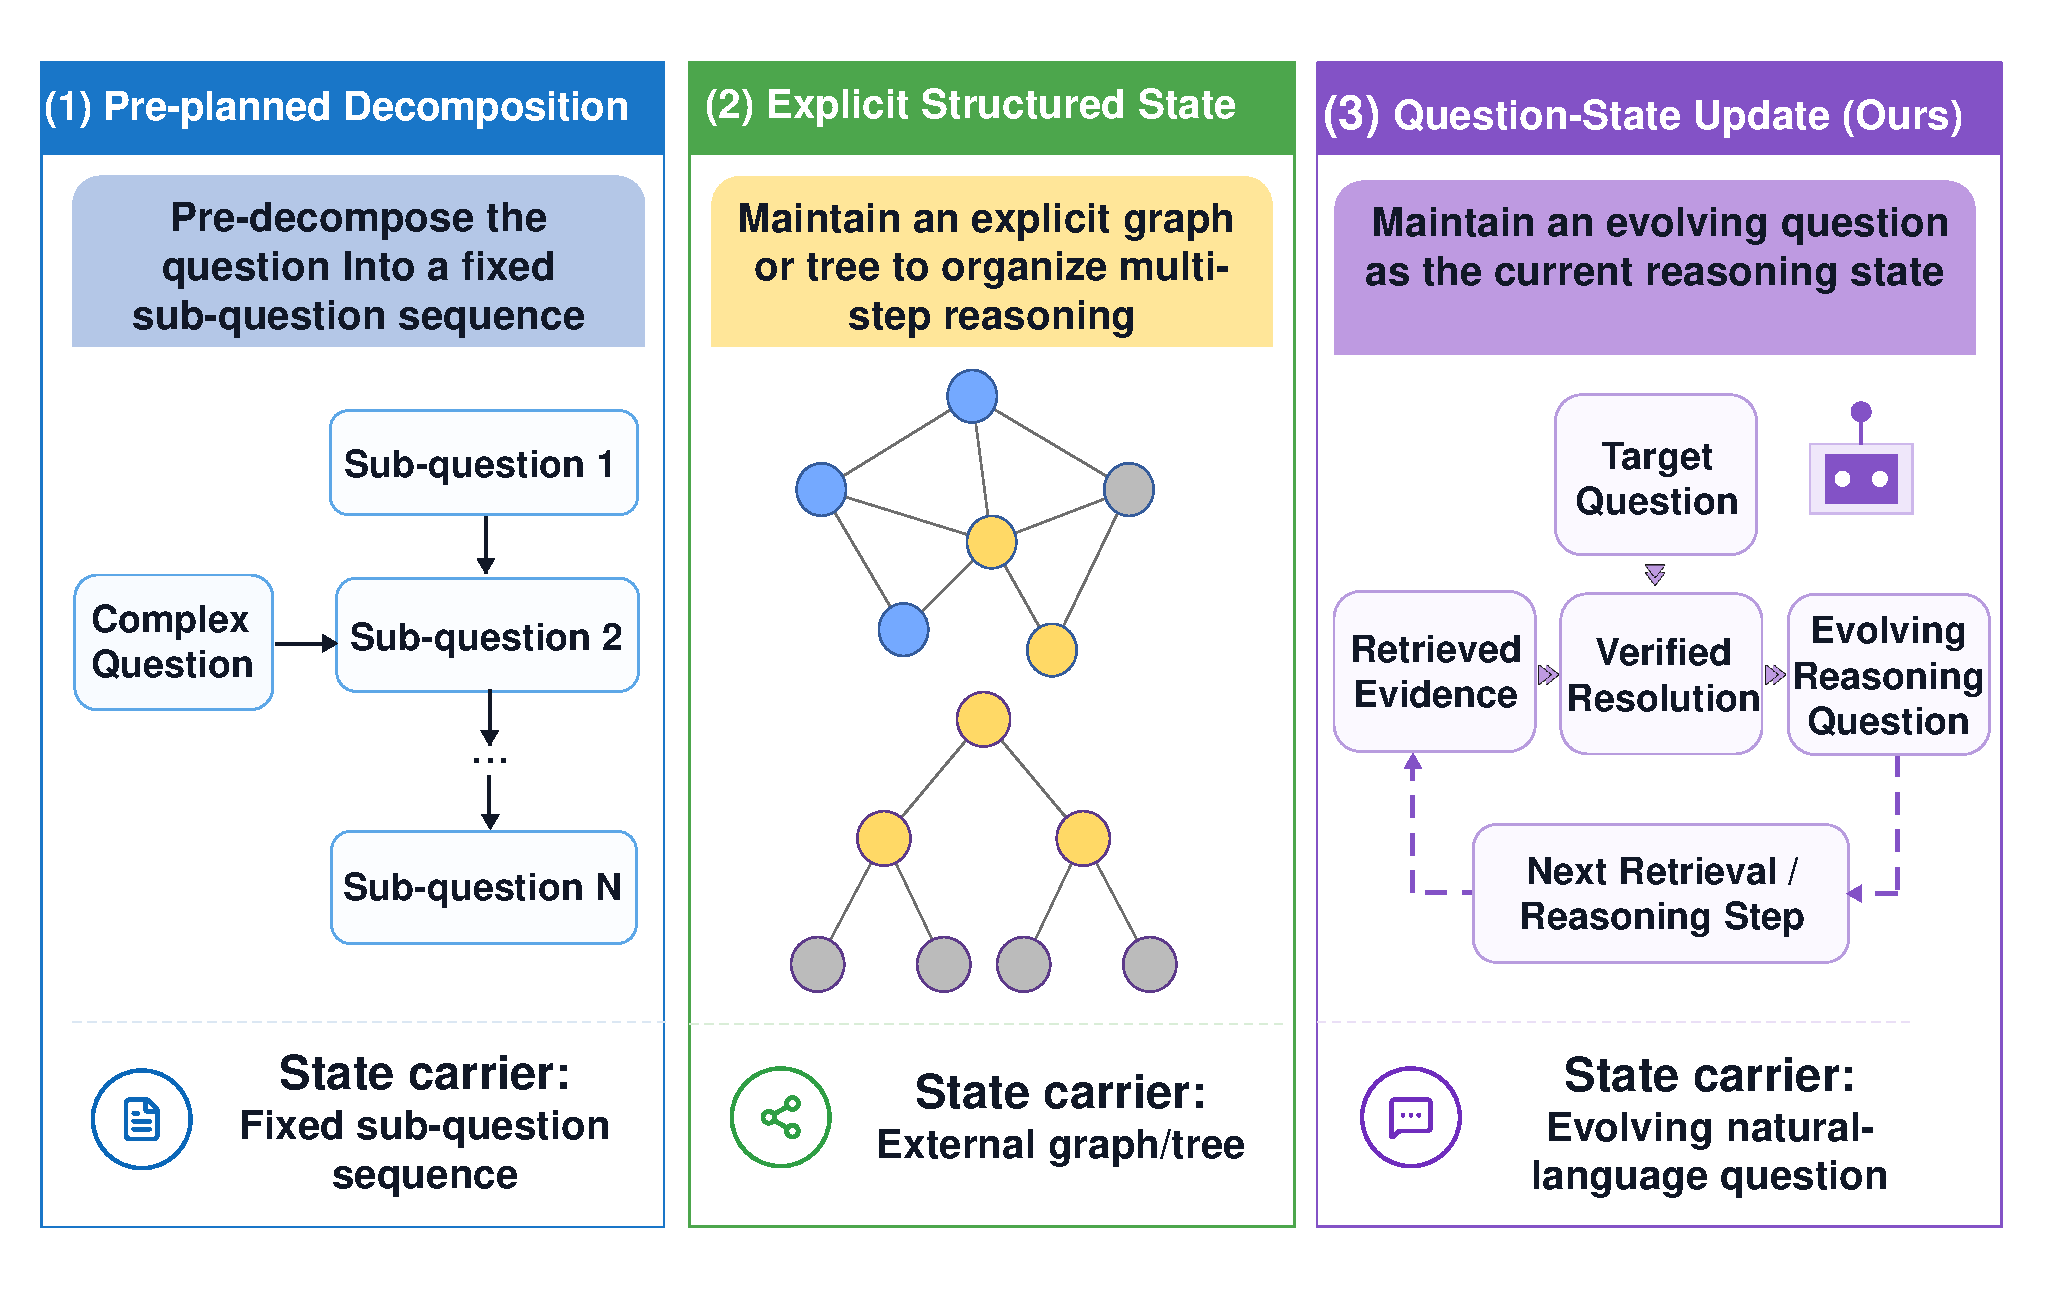
\includegraphics[width=\columnwidth]{figures/figure1.pdf}
		\caption{多跳 RAG 中三种推理状态载体的概念比较：固定子问题序列、显式图/树状态，以及 QSR-RAG 中持续演化的自然语言问题。}
		\label{fig:state-carriers}
	\end{figure}

	\section{QSR-RAG 方法}

	\subsection{状态表示与迭代}
	给定一个多跳问题 $Q$ 和文档集合 $D$，QSR-RAG 维护三个持久对象：固定的目标问题 $Q^{(0)}$、持续演化的推理问题 $Q^{(t)}$，以及已验证解答记忆 $M^{(t)}$。局部问题 $q^{(t)}$ 只在当前轮次内使用。初始时，两类问题都等于 $Q$。每个被接纳的中间解答表示为 $r_i=\langle q_i,z_i,a_i,E_i\rangle$，其中 $z_i$、$a_i$ 和 $E_i$ 分别表示解答目标、局部答案以及直接支撑该答案的证据。

	$M^{(t)}$ 和 $Q^{(t)}$ 都会跨轮次保留，但二者作用不同。记忆存储被接受的事实，例如“《The Feminine Mystique》的作者 $=$ Betty Friedan”。推理问题则把这些事实重新放回当前任务中，从而保留它们对尚未解析的关系和最终答案空间的影响。记忆提供事实记录，而 $Q^{(t)}$ 显式记录这些事实如何改变任务表述。因此，我们并不把推理问题视为记忆的替代品；它是在记忆条件下对当前任务的表达。它也不必是尽可能短的“剩余问题”：当比较结构或答案空间语义需要保留时，保留部分原始措辞反而更加安全。

	问题生成器根据当前推理问题、累计记忆和局部问题历史 $H^{(t)}$ 生成下一条信息需求：
	\begin{equation}
		q^{(t)}=G\!\left(Q^{(t)},M^{(t)},H^{(t)}\right).
		\label{eq:generator}
	\end{equation}
	获得并验证新的局部解答 $R^{(t)}$ 后，完整 QSR-RAG 执行更新：
	\begin{equation}
		Q^{(t+1)}=U\!\left(Q^{(t)},R^{(t)}\right),
		\label{eq:update}
	\end{equation}
	并将通过验证的结果加入 $M^{(t+1)}$。局部问题在当前轮结束后不再保留，而更新后的 $Q^{(t+1)}$ 会作为下一轮的输入。仅记忆对照仍保留式~\ref{eq:generator} 中记忆和局部问题历史的影响，但移除式~\ref{eq:update}；由此可以单独隔离“持久问题状态更新”的作用。

	\subsection{基于证据的局部解答与状态准入}
	\begin{figure*}[t]
		\centering
		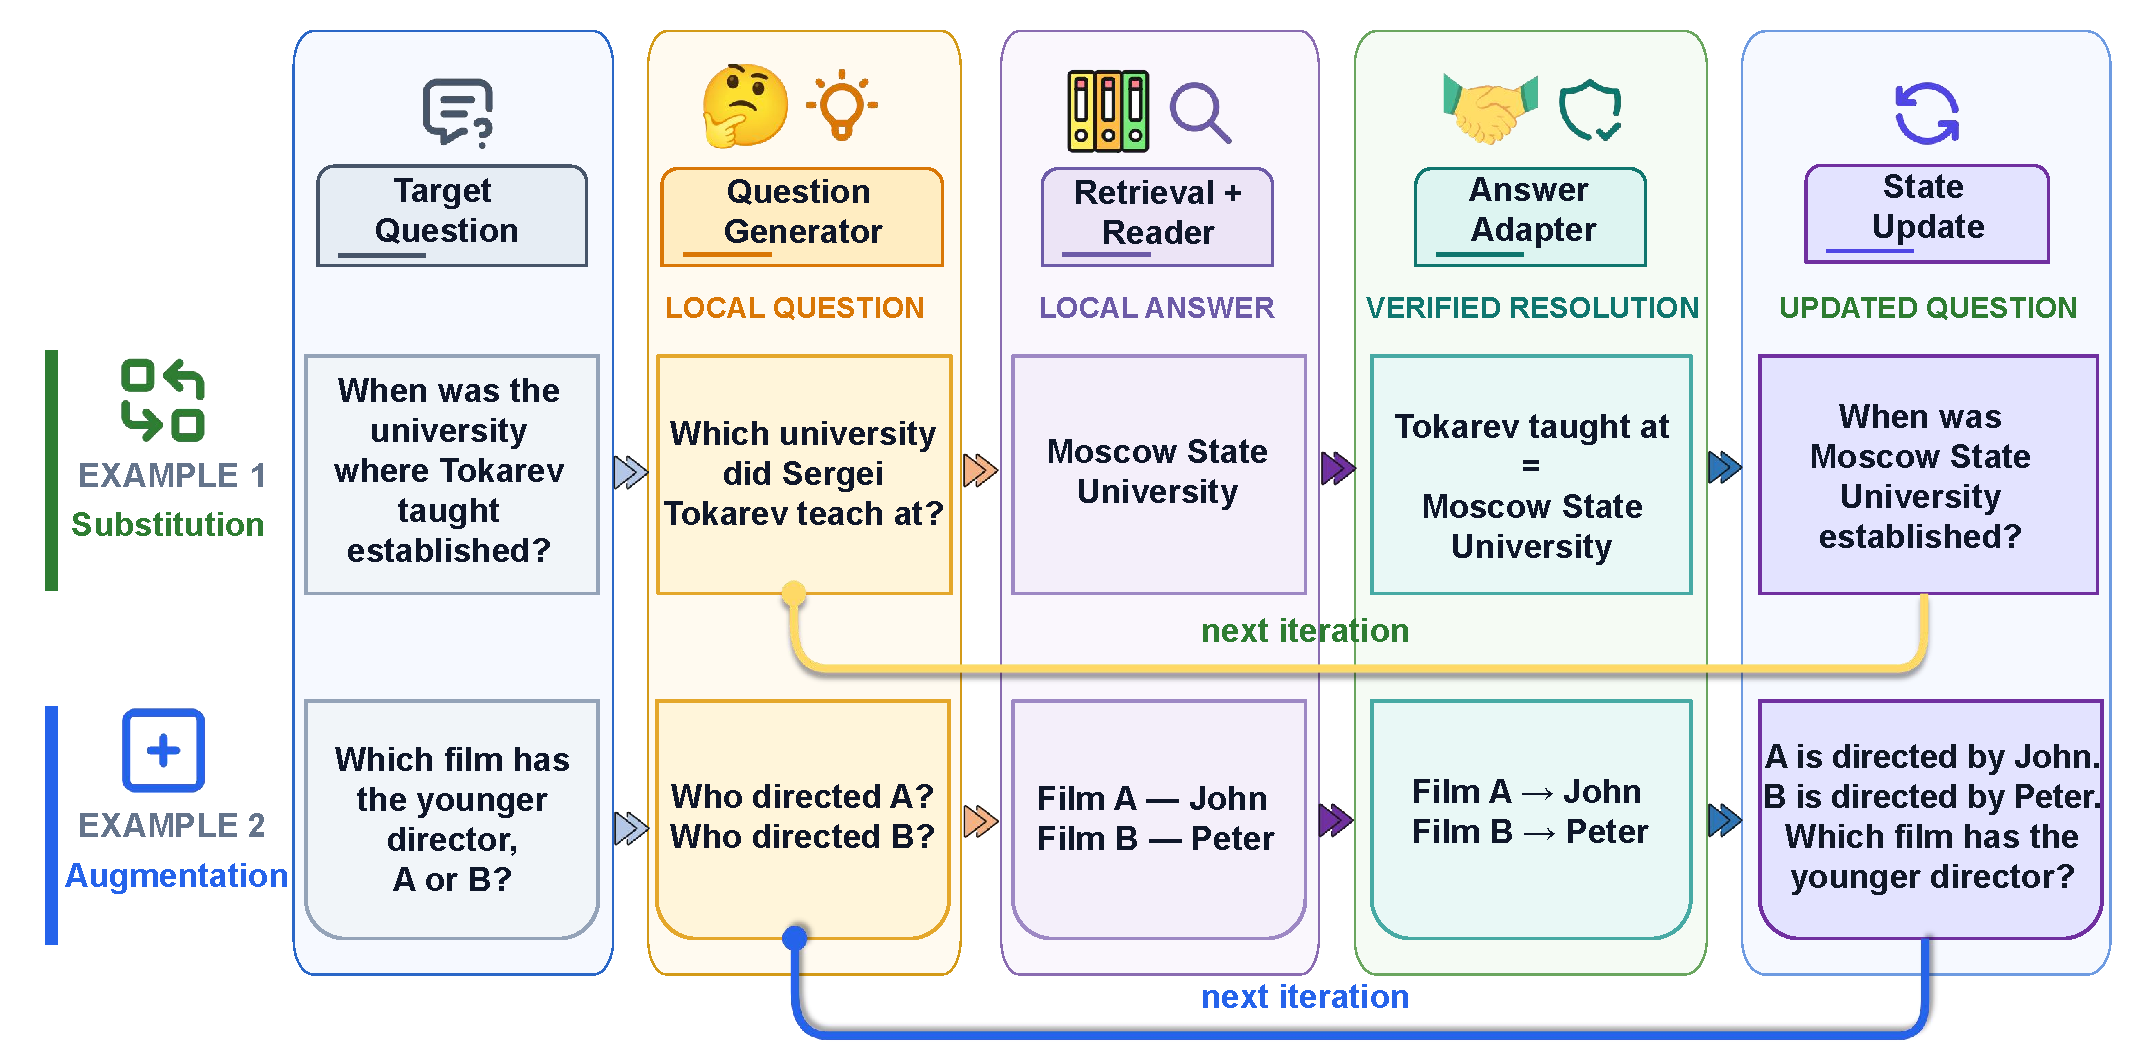
\includegraphics[width=\textwidth]{figures/figure2.pdf}
		\caption{QSR-RAG 中基于证据的问题状态演化过程，并给出替换与增强两种更新操作的示例。}
		\label{fig:qsr-workflow}
	\end{figure*}

	如图~\ref{fig:qsr-workflow} 所示，每一轮首先从当前推理问题中定位一个尚未解决的信息缺口。对于隐藏实体依赖，生成器按照由内向外的顺序，优先解析阻塞外层关系的最内层未知项。例如，当一个外层属性问题依赖某个尚未确定的人物或组织时，系统首先询问该隐藏实体，而不是直接猜测外层答案。局部问题尽可能从当前问题中出现的实体，或已在已验证解答记忆中确认的实体出发，并且一次只跨越一个尚未解析的关系。生成器不会预先生成完整推理计划，也不会直接回答最终问题。

	每个局部问题首先使用 BGE-M3 检索文档。检索到的文档经过共享的重排序流程后，由局部阅读器生成候选答案。随后，答案适配器检查两个条件：候选答案是否真正填补了当前解答目标，以及检索证据是否直接支持该目标关系。第二个检查十分重要，因为答案字符串可能出现在证据中，却并不支持当前正在解析的关系。只有通过检查的结果才会写入已验证解答记忆并用于问题状态更新。这里的“已验证”只是模型基于检索证据作出的操作性判断，并不构成形式化的正确性保证。如果验证失败，当前实现不会使用该候选结果来推进状态。检索、重试和停止策略的细节见附录~\ref{app:implementation}。

	\subsection{问题状态重写}
	状态更新器只修改推理问题，目标问题始终保持不变。每个被接受的解答都会被写回当前任务，同时尽量保持最终信息需求、候选对象身份、逻辑操作、尚未解析的外层关系以及答案空间不变。QSR-RAG 使用两种互补操作。

	\paragraph{替换（Substitution）。}
	当某个已验证解答识别出后续推理所需的隐藏实体时，与解答目标对齐的描述会被绑定到该实体。例如，如果 $\text{John 的父亲}=\text{Tom}$，那么“John 的父亲是什么国籍？”可以改写为“Tom 是什么国籍？”这样，已经解决的实体依赖就变成了显式实体提及，使下一条局部问题可以直接围绕该实体执行。

	\paragraph{增强（Augmentation）。}
	对于比较、选择、布尔等问题，直接替换可能改变答案空间。例如，在“Film A 和 Film B 中，哪部电影的导演更年轻？”这一问题中，如果把电影名称直接替换为导演姓名，答案空间就会从 Film A/B 变成 John/Peter。因此，QSR-RAG 保留原始候选项和决策结构，并把“Film A 由 John 执导”“Film B 由 Peter 执导”等已验证事实作为前提加入推理问题。完整系统根据当前解答在语义上的作用选择替换或增强。如果状态更新器的安全检查认为候选重写会违反任务约束，则保持当前问题不变。由于该检查由模型驱动，它只能提供操作层面的语义约束，而不能形式化地保证关系一定被完整保留。

	\subsection{最终答案生成}
	当生成器不再产生新的信息缺口、达到最大轮次预算，或当前解答未能通过验证时，最终阅读器将目标问题、最终推理问题、累计的已验证解答以及有效证据组合起来：
	\begin{equation}
		y=\operatorname{Reader}\!\left(Q^{(0)},Q^{(T)},M^{(T)},E^{*}\right).
		\label{eq:final-reader}
	\end{equation}
	其中，$Q^{(0)}$ 用于确保答案始终锚定原始任务及其答案空间；$Q^{(T)}$ 提供已经纳入中间解答后的任务上下文；$M^{(T)}$ 与 $E^{*}$ 则共同保留已接纳的事实及其支撑证据。

	\section{实验设置}

	\subsection{数据集、基线与实现}
	我们在 HotpotQA、2WikiMultiHopQA 和 MuSiQue 上评估 QSR-RAG \citep{yang2018hotpotqa,ho2020twowiki,trivedi2022musique}。对每个数据集，我们使用随机种子 43 抽取 500 个问题，并分别使用 GPT-4o-mini 和 Qwen3-8B 进行评测，其中 Qwen3-8B 采用非思考模式，因此构成六个主要实验设置。基线包括 Direct RAG、Self-Ask、Iter-RetGen、ProbTree、IRCoT-style、ChainRAG 和 DEC。由于我们未能找到可验证的官方实现，UniRAG 仅用于概念层面的比较。为了测试结果对随机抽取评测集组成的稳健性，我们还分别针对 GPT-4o-mini 和 Qwen3-8B，使用样本选择随机种子 44 和 2027 重新运行 QSR-RAG。除此之外，我们还在 seed-43 的样本上使用 Qwen3.5-Plus 评估 QSR-RAG，以考察该框架能否从更强的主干模型中获益。这些补充实验统一报告在附录~\ref{app:robustness} 中，不纳入正文主基线表。

	\textbf{统一检索后端。}
	为了控制检索器质量这一混杂因素，我们重新实现的所有方法都使用相同语料库和相同的逐查询检索流程：BGE-M3 + FAISS 稠密检索 top-200 $\rightarrow$ bge-reranker-v2-m3 重排序到 top-60 $\rightarrow$ 半径为 1 的句子窗口重排序 $\rightarrow$ 保留 top-20 窗口。每种方法仍保留自身的查询生成、问题分解、迭代调度、推理状态与停止逻辑。因此，主要比较关注的是共享检索基础设施下的推理和检索控制策略，而不是检索器本身的差异；主表中的基线结果应被理解为我们实验环境中的受控重实现。QSR-RAG 每个问题最多执行四轮，每轮最多生成两个处于相同依赖层级的局部问题。完整实现与复现实验细节见附录~\ref{app:implementation}，提示词协议见附录~\ref{app:prompts}。

	\subsection{评测指标与统计检验}
	主要评测指标为精确匹配（Exact Match, EM）和 token 级 F1。支撑文档/句子召回率与资源使用量作为补充分析。对于完整版与仅记忆设置之间的 F1 差异，我们使用按样本配对的 bootstrap 95\% 置信区间以及双侧配对随机化检验，并对三个数据集级别的 $p$ 值执行 Holm 校正。EM 使用精确 McNemar 检验。除逐数据集检验外，我们还报告三个数据集上的等权分层聚合分析，以总结跨数据集的平均趋势。统计过程与资源指标定义详见附录~\ref{app:state-significance} 和附录~\ref{app:efficiency}。

	\subsection{消融设置}
	\label{sec:ablation-setup}
	问题状态更新消融在每个数据集固定抽取的 300 个样本上使用 GPT-4o-mini 进行。\textbf{仅记忆（Memory-only）}保留问题生成器、检索器、局部阅读器、答案适配器、已验证解答记忆、局部问题历史和最终阅读器，但固定 $Q^{(t)}=Q^{(0)}$；它仍会动态生成
	\begin{equation}
		q^{(t)}_{\mathrm{Mem}}=G\!\left(Q^{(0)},M^{(t)},H^{(t)}\right).
		\label{eq:memory-only}
	\end{equation}
	因此，仅记忆设置仍然可以利用记忆改变后续局部问题和检索轨迹；它只是停止更新持久的推理问题。我们还比较 \textbf{仅替换（Substitution Only）}、\textbf{仅增强（Augmentation Only）}和能够在两种操作之间自适应选择的 \textbf{完整 QSR-RAG（Full QSR-RAG）}。其余核心组件均保持一致。

	答案适配器消融在相同的 300 个样本上比较 \textbf{完整（Full）}、\textbf{证据不可见（Evidence-Blind）}和\textbf{无验证（No Verification）}三种设置。这三种条件共享同一个状态更新器和最终阅读器，只在两个方面存在差异：中间候选答案进入持久状态之前是否接受目标一致性检查，以及验证器是否能够看到检索证据。这样可以区分“目标一致性”与“证据必须直接支持目标关系”这两个额外要求。完整组件定义见附录~\ref{app:adapter-details}。

	\section{实验结果}

	\subsection{主要结果}
	表~\ref{tab:main-results} 给出了主要结果。在两个主干模型和三个数据集构成的六种设置中，QSR-RAG 在所有对比方法中都取得了最高的 EM/F1。这说明在样本一致、检索后端统一，并且每个设置中使用相同生成主干模型的条件下，完整系统具有较强竞争力。问题状态重写本身的贡献将在下文通过仅记忆消融进行更直接的检验。使用不同样本选择随机种子以及更强的 Qwen3.5-Plus 主干模型进行的补充实验还显示了较一致的样本层面稳健性，以及随主干模型能力增强而提升的趋势；详细结果见附录~\ref{app:robustness}。

	\begin{table*}[t]
		\centering
		\caption{在统一检索后端下，三个多跳问答数据集上的主要结果（\%，每个数据集 $n=500$）。}
		\label{tab:main-results}
		\small
		\setlength{\tabcolsep}{4.2pt}
		\begin{tabular}{lrrrrrr}
			\toprule
			& \multicolumn{2}{c}{HotpotQA} & \multicolumn{2}{c}{2WikiMultiHopQA} & \multicolumn{2}{c}{MuSiQue}\\
			\cmidrule(lr){2-3}\cmidrule(lr){4-5}\cmidrule(lr){6-7}
			方法 & EM & F1 & EM & F1 & EM & F1\\
			\midrule
			\multicolumn{7}{l}{\textbf{(a) GPT-4o-mini}}\\
			Direct RAG          & 50.80 & 65.75 & 41.40 & 47.84 & 23.40 & 35.85\\
			Self-Ask            & 38.20 & 53.82 & 25.00 & 35.77 & 24.40 & 35.67\\
			Iter-RetGen         & 30.80 & 50.22 & 42.20 & 55.17 & 30.60 & 46.32\\
			ProbTree            & 42.80 & 57.12 & 36.60 & 42.23 & 16.40 & 26.37\\
			IRCoT-style         & 55.40 & 70.47 & 57.60 & 72.08 & 34.60 & 51.02\\
			ChainRAG w/ SubQ    & 45.60 & 61.48 & 44.80 & 50.22 & 32.80 & 45.40\\
			ChainRAG w/o SubQ   & 50.20 & 65.06 & 42.80 & 48.72 & 31.20 & 41.67\\
			DEC                 & 38.20 & 55.54 & 41.60 & 53.91 & 28.80 & 38.19\\
			\textbf{QSR-RAG}    & \textbf{57.60} & \textbf{73.65} & \textbf{64.80} & \textbf{74.19} & \textbf{42.00} & \textbf{55.35}\\
			\midrule
			\multicolumn{7}{l}{\textbf{(b) Qwen3-8B}}\\
			Direct RAG          & 46.80 & 62.26 & 38.60 & 44.32 & 21.40 & 34.25\\
			Self-Ask            & 44.80 & 58.87 & 29.60 & 37.59 & 18.60 & 28.39\\
			Iter-RetGen         & 50.00 & 66.25 & 36.40 & 58.49 & 29.80 & 42.24\\
			ProbTree            & 21.00 & 32.80 & 28.40 & 32.72 &  6.60 & 16.14\\
			IRCoT-style         & 52.60 & 66.98 & 61.40 & 69.99 & 30.20 & 40.65\\
			ChainRAG w/ SubQ    & 39.40 & 55.50 & 41.00 & 47.74 & 22.60 & 35.22\\
			ChainRAG w/o SubQ   & 41.80 & 56.74 & 37.80 & 44.49 & 20.40 & 32.91\\
			DEC                 & 42.00 & 55.29 & 43.00 & 49.36 & 24.00 & 32.87\\
			\textbf{QSR-RAG}    & \textbf{57.40} & \textbf{72.25} & \textbf{62.60} & \textbf{71.88} & \textbf{35.20} & \textbf{48.13}\\
			\bottomrule
		\end{tabular}
	\end{table*}

	在 GPT-4o-mini 下，QSR-RAG 相比最强基线，在 HotpotQA、2WikiMultiHopQA 和 MuSiQue 上的 F1 分别提升 3.18、2.11 和 4.33 个百分点。在 Qwen3-8B 下，对应提升分别为 5.27、1.89 和 5.89 个百分点。对六种设置取平均后，QSR-RAG 相比最强基线领先 4.63 个 EM 点和 3.78 个 F1 点。在 GPT-4o-mini 下，QSR-RAG 的平均 F1 为 67.73，每个问题平均消耗 20.47k tokens。与相同主干下的 IRCoT-style 相比，它的平均 F1 提升 3.21 个百分点，同时 token 使用量减少 52.8\%，但需要更多 LLM 调用。因此，我们将这一结果解释为较有利的“准确率--token”权衡，而不是声称 QSR-RAG 在所有资源指标上成本最低。完整资源消耗结果见附录~\ref{app:efficiency}。

	\subsection{问题状态重写消融}
	表~\ref{tab:ablation} 比较了仅记忆、两种单一更新策略以及完整 QSR-RAG。由于仅记忆设置已经能够利用累计记忆动态改变后续局部问题，因此它是一个比简单固定查询基线更强的对照。该对照直接检验：当事实记忆已经支持动态查询生成时，额外维护一个持久的完整问题状态是否仍然能够带来收益。

	\begin{table*}[t]
		\centering
		\caption{问题状态重写消融结果（GPT-4o-mini，每个数据集 $n=300$，\%）。}
		\label{tab:ablation}
		\small
		\setlength{\tabcolsep}{5pt}
		\begin{tabular}{lrrrrrr}
			\toprule
			& \multicolumn{2}{c}{HotpotQA} & \multicolumn{2}{c}{2WikiMultiHopQA} & \multicolumn{2}{c}{MuSiQue}\\
			\cmidrule(lr){2-3}\cmidrule(lr){4-5}\cmidrule(lr){6-7}
			方法 & EM & F1 & EM & F1 & EM & F1\\
			\midrule
			仅记忆（Memory-only）       & 58.00 & 74.40 & 62.33 & 71.96 & 40.33 & 53.88\\
			仅替换（Substitution Only） & 58.00 & 74.14 & 61.67 & 70.40 & 40.67 & 54.29\\
			仅增强（Augmentation Only） & 58.00 & 74.11 & 62.33 & 71.37 & 38.67 & 52.72\\
			\textbf{完整 QSR-RAG} & \textbf{60.33} & \textbf{76.14} & \textbf{65.33} & \textbf{75.36} & \textbf{42.33} & \textbf{55.98}\\
			\bottomrule
		\end{tabular}
	\end{table*}

	相较于仅记忆设置，完整版在 HotpotQA 上的 EM/F1 提升 2.33/1.74，在 2WikiMultiHopQA 上提升 3.00/3.40，在 MuSiQue 上提升 2.00/2.10，平均提升为 2.44 EM 和 2.41 F1。三个数据集上的 F1 差异均为正，说明显式更新推理问题能够在已有记忆之外提供额外的端到端收益。2WikiMultiHopQA 上 $+3.40$ 的 F1 增益在 Holm 校正后仍然显著（$p_{\mathrm{Holm}}=0.0112$），而 HotpotQA 和 MuSiQue 的置信区间跨过 0。等权分层聚合分析得到 $\Delta$F1=$+2.41$、95\% CI $[+0.75,+4.10]$，且 $p=0.0042$。完整统计结果见附录~\ref{app:state-significance}。

	2WikiMultiHopQA 还提供了一个有用的诊断视角。表~\ref{tab:2wiki-recall-diagnostic} 对比了答案质量与金标准支撑证据召回率。完整版检索到的标注支撑证据略少于仅记忆设置，却取得了更高的 EM/F1。因此，该数据集上的增益不能简单归因于“检索到了更多金标准证据”，而更符合这样一种解释：差异来自中间事实在后续推理中的组织与使用方式。

	\begin{table}[t]
		\centering
		\caption{2WikiMultiHopQA 上完整版与仅记忆设置的答案质量和支撑证据召回率（GPT-4o-mini，$n=300$，\%）。}
		\label{tab:2wiki-recall-diagnostic}
		\small
		\setlength{\tabcolsep}{3.6pt}
		\begin{tabular}{lrrrr}
			\toprule
			设置 & EM & F1 & 文档召回率 & 句子召回率\\
			\midrule
			仅记忆 & 62.33 & 71.96 & \textbf{98.17} & \textbf{93.75}\\
			\textbf{完整版} & \textbf{65.33} & \textbf{75.36} & 97.83 & 92.75\\
			\bottomrule
		\end{tabular}
	\end{table}

	在三个数据集上，完整版也都不劣于任一单一更新策略。如果系统只能使用替换或只能使用增强，那么不同结构的问题都被迫采用同一种变换。完整版则根据当前解答是否能够安全地绑定到某个实体，以及替换是否会改变答案空间来选择操作。下面的操作分布提供了该路由机制的行为视角。

	\subsection{状态转移行为分析}
	不同数据集上被接受的更新操作比例差异明显：在 HotpotQA 上，替换/增强占 \textbf{76.7\%/23.3\%}；在 2WikiMultiHopQA 上占 \textbf{64.5\%/35.5\%}；在 MuSiQue 上占 \textbf{92.5\%/7.5\%}。MuSiQue 主要由实体绑定主导，而 2WikiMultiHopQA 更频繁触发增强，说明该数据集中系统更常遇到必须保留候选对象和原始答案空间的更新情形。不同数据集上的路由分布差异较大，表明两种操作在真实轨迹中承担了不同的状态转换作用。结合表~\ref{tab:ablation}，这些结果支持“根据问题结构选择更新方式”，而不是声称某一种操作普遍更优。精确计数见附录~\ref{app:rewrite-behavior}。

	\subsection{答案适配器消融：准确率与轨迹效率}
	\begin{table}[t]
		\centering
		\caption{答案适配器消融的 F1 结果（GPT-4o-mini，$n=300$，\%）。}
		\label{tab:adapter-ablation}
		\small
		\setlength{\tabcolsep}{3.8pt}
		\begin{tabular}{lrrr}
			\toprule
			设置 & Hotpot & 2Wiki & MuSiQue\\
			\midrule
			证据不可见 & 71.79 & 73.79 & 50.89\\
			无验证 & 73.48 & 74.22 & 55.81\\
			\textbf{完整版} & \textbf{76.14} & \textbf{75.36} & \textbf{55.98}\\
			\bottomrule
		\end{tabular}
	\end{table}

	完整版相较于无验证设置，平均 F1 提升 1.33 个百分点；相较于证据不可见设置，平均 F1 提升 3.67 个百分点。在 MuSiQue 上，完整版与无验证设置之间仅相差 0.17 F1，因此答案适配器的作用不能只用最终准确率衡量。证据不可见与完整版之间的差距也表明：让验证器看到检索证据，可以提高状态准入的质量。

	验证机制也会改变推理轨迹。三个数据集取平均后，完整版将解答轮数从 2.22 降至 2.03（$-8.4\%$），检索调用次数从 4.69 降至 4.56（$-2.9\%$），LLM 调用次数从 12.07 降至 11.57（$-4.2\%$）。在 MuSiQue 上，F1 基本不变（55.98 vs.\ 55.81），但轮数/检索调用/LLM 调用分别从 2.43/4.68/12.61 降至 2.04/4.36/11.47。这一现象与以下解释一致：适配器阻止部分未通过证据或目标检查的候选结果传播到更长的轨迹中；不过，仅凭轨迹统计并不能证明每一次被避免的检索都是无用的。由于证据检查本身也会消耗上下文，总 token 使用量基本没有变化。因此，我们更保守地得出结论：验证使推理轨迹更短、更受控，而不是降低了所有成本指标。完整统计结果见附录~\ref{app:adapter-details}。

	\section{结论}
	QSR-RAG 将固定的目标问题、持续更新的推理问题、已验证解答记忆以及临时的局部问题区分开来，并利用自然语言问题本身在跨轮次过程中保存任务进展。状态通过两种互补操作进行更新：替换用于绑定已经解析出的隐藏实体；增强则在需要保留原始候选项与答案空间时，将已验证事实作为前提加入问题。在三个数据集和两个主干模型上，完整系统在所有对比方法中均取得最高的 EM/F1。相较于仍然能够利用记忆动态生成局部问题的仅记忆设置，完整版平均提升 2.44 个 EM 点和 2.41 个 F1 点。在 2WikiMultiHopQA 上，尽管完整版的金标准证据召回率略低，但答案质量仍然更高，这进一步说明问题状态更新并不等价于简单地检索更多证据。答案适配器控制哪些中间结果能够进入持久状态，并在部分设置中缩短后续推理轨迹。

	\section{局限性}
	QSR-RAG 的信息缺口发现、局部阅读器、答案适配器和状态更新器都依赖底层语言模型。因此，对关系的错误理解、指代解析错误、状态重写错误或局部目标设定错误，都可能使后续轨迹偏离正确方向。所谓“已验证解答”只意味着当前证据支持当前局部问题的答案，并且该答案填补了对应解答目标；它并不能保证状态写回后，或下一轮的局部目标，仍然与原始任务保持一致。在附录~\ref{app:cases} 的失败轨迹中，系统在第 2 轮已经获得金标准答案，但随后进行的状态写回没有保留原始条件关系，从而生成了语义发生漂移的推理问题。下一轮生成器进一步扩大了条件性雇佣关系的含义。之后的答案虽然得到了新局部目标对应证据的支持，却最终使最终阅读器给出错误答案。因此，证据约束能够限制局部答案是否可信，但仅靠它无法保证状态转移保持原始关系，也无法阻止目标设定漂移。此外，保守的拒绝策略还可能过早终止较长的推理链。

	当前实验检索的是各基准开发集所包含文档的并集，而不是 Wikipedia 规模的语料库。更大、更嘈杂的文档集合会增加实体歧义、检索难度和时延，因此在这种场景下，问题状态更新是否仍能保持相同收益尚待验证。三个数据集还使用了不同的上下文示例；统一示例设置、零样本设置以及跨领域泛化能力都需要进一步研究。最后，QSR-RAG 并非在所有资源指标上都是成本最低的方法。检索缓存、批量化局部问题与验证，以及更紧凑的状态更新，都是自然的效率优化方向 \citep{yang2026compact}。

	\bibliography{qsr_rag}

	% Keep consecutive full-width appendix tables grouped near the top of
	% float-only pages instead of stretching them across the full page height.
	\makeatletter
	\setlength{\@dblfptop}{0pt}
	\setlength{\@dblfpsep}{12pt}
	\setlength{\@dblfpbot}{0pt plus 1fil}
	\makeatother
	\appendix

	\section{实现与检索细节}
	\label{app:implementation}

	主要实验使用随机种子 43，从 HotpotQA、2WikiMultiHopQA 和 MuSiQue 的开发集中各随机抽取 500 个问题，并确保所有方法都在同一份样本列表上评测。对于临时的服务提供商或网络故障，统一采用相同的重试策略；若重试后仍无法获得有效预测，该样本仍保留在分母中，并记为 EM/F1=0。问题状态更新和答案适配器消融均使用 GPT-4o-mini，在每个数据集固定的 300 个样本子集上进行（seed 43）。补充稳健性实验采用相同的 QSR-RAG 与检索配置，仅将样本选择随机种子改为 44 和 2027；在同一个 seed 下，两个原始主干模型使用相同的问题 ID。Qwen3.5-Plus 实验使用 seed-43 的样本列表。

	\paragraph{统一检索后端与基线复现。}
	我们控制性重实现中的所有方法都共享完全相同的检索基础设施。我们使用 BGE-M3 + FAISS 进行单通道稠密检索 \citep{chen2024bgem3,johnson2021faiss}。每个索引都由对应基准完整开发集中出现的文档并集构建：HotpotQA 包含 66,581 篇文档，2WikiMultiHopQA 包含 56,686 篇，MuSiQue 包含 21,098 篇。无论输入是 Direct RAG 的原始问题，还是迭代方法生成的检索查询，都采用相同的逐查询流程：先稠密检索 top-200 文档，再使用 bge-reranker-v2-m3 重排到 top-60，之后构造半径为 1 的句子窗口并再次重排序，最终为对应阅读器保留 top-20 窗口。我们不会为任何单独基线分配更强或更弱的检索器，也没有任何方法获得额外检索通道或多通道融合。

	被标准化的只有检索基础设施。每种方法仍然保留自身关于\emph{检索什么、何时继续检索以及如何携带推理历史}的机制。Self-Ask 保留中间问题生成；IRCoT-style 保留推理--检索交错机制；Iter-RetGen 保留检索--生成循环；ProbTree 保留其显式推理结构；ChainRAG 保留子问题/渐进式重写逻辑；DEC 则保留带上下文感知查询增强的问题分解。这样做的目的，是控制检索器质量这一混杂因素，在统一检索后端下比较查询/推理控制策略，而不是复现原论文中彼此异构的检索器组合。因此，主表中的基线得分应理解为我们实验环境下的受控重实现结果。

	\begin{table}[t]
		\centering
		\caption{主要实验中被统一控制的因素与方法特定因素。}
		\label{tab:baseline-control}
		\small
		\setlength{\tabcolsep}{3.2pt}
		\begin{tabular}{p{0.38\columnwidth}p{0.50\columnwidth}}
			\toprule
			项目 & 设置 \\
			\midrule
			语料库 / 文档索引 & 所有方法共享 \\
			稠密检索器 & BGE-M3 + FAISS，共享 \\
			文档重排序器 & bge-reranker-v2-m3，共享 \\
			检索深度 & top-200 $\rightarrow$ top-60 $\rightarrow$ top-20 窗口，共享 \\
			生成主干模型 & 每个实验设置内共享 \\
			查询 / 分解逻辑 & 方法特定 \\
			迭代 / 推理状态 & 方法特定 \\
			停止逻辑 & 方法特定 \\
			\bottomrule
		\end{tabular}
	\end{table}

	QSR-RAG 对每个问题最多允许四轮局部解答，每轮最多生成两个位于相同依赖层级、彼此独立的局部问题。三个数据集共享相同的核心系统指令、决策顺序和输出模式。只有上下文演示样例会被替换，用于展示各基准中常见的问题形式；这些示例既不包含金标准答案，也不包含金标准支撑证据。核心提示词和输出协议见附录~\ref{app:prompts}。

	主要答案指标为精确匹配（EM）和 token 级 F1；支撑文档/句子召回率的完整定义见附录~\ref{app:evidence-recall}。资源使用量定义为每个问题所有 prompt token 与 completion token 的总和。完整版与仅记忆设置之间的统计检验细节见附录~\ref{app:state-significance}。



	\section{样本选择随机种子稳健性与更强主干模型实验}
	\label{app:robustness}

	主要结果使用随机种子 43，从每个开发集中随机抽取 500 个问题。为了检验报告的 QSR-RAG 性能是否强烈依赖于这一特定样本组成，我们分别对 GPT-4o-mini 和 Qwen3-8B 使用样本选择随机种子 44 和 2027，重新运行完整 QSR-RAG 评测。改变随机种子会改变被抽取的问题，因此该实验应被理解为对“评测集组成”的稳健性检验，而不是在完全相同样本上重复进行随机解码。同一个 seed 下，两个主干模型使用相同的问题 ID，并采用与主实验一致的检索流程和 QSR-RAG 配置。

	\begin{table*}[t]
		\centering
		\caption{QSR-RAG 在每个数据集三组随机 500 问题样本上的结果（\%，seed 为 43、44 和 2027）。``平均''表示对应 seed 下 HotpotQA、2WikiMultiHopQA 和 MuSiQue 三个数据集结果的算术平均。}
		\label{tab:seed-robustness}
		\scriptsize
		\setlength{\tabcolsep}{3.6pt}
		\resizebox{\textwidth}{!}{%
			\begin{tabular}{llrrrrrrrr}
				\toprule
				主干模型 & Seed & \multicolumn{2}{c}{HotpotQA} & \multicolumn{2}{c}{2WikiMultiHopQA} & \multicolumn{2}{c}{MuSiQue} & \multicolumn{2}{c}{平均}\\
				\cmidrule(lr){3-4}\cmidrule(lr){5-6}\cmidrule(lr){7-8}\cmidrule(lr){9-10}
				& & EM & F1 & EM & F1 & EM & F1 & EM & F1\\
				\midrule
				GPT-4o-mini & 43   & 57.60 & 73.65 & 64.80 & 74.19 & 42.00 & 55.35 & 54.80 & 67.73\\
				GPT-4o-mini & 44   & 60.40 & 76.43 & 66.80 & 74.59 & 38.00 & 52.04 & 55.07 & 67.69\\
				GPT-4o-mini & 2027 & 57.20 & 72.87 & 62.80 & 73.01 & 38.20 & 54.73 & 52.73 & 66.87\\
				\midrule
				Qwen3-8B & 43   & 57.40 & 72.25 & 62.60 & 71.88 & 35.20 & 48.13 & 51.73 & 64.09\\
				Qwen3-8B & 44   & 58.80 & 74.00 & 67.60 & 74.87 & 33.40 & 48.34 & 53.27 & 65.74\\
				Qwen3-8B & 2027 & 56.00 & 70.60 & 62.80 & 72.96 & 34.20 & 51.12 & 51.00 & 64.89\\
				\bottomrule
		\end{tabular}}
	\end{table*}

	在三个样本选择随机种子下，GPT-4o-mini 的跨数据集平均 F1 分别为 67.73、67.69 和 66.87；Qwen3-8B 分别为 64.09、65.74 和 64.89。由于每个 seed 对应的 500 个问题不同，单个数据集的得分会发生变化，但三个随机样本上的跨数据集平均值彼此接近。这说明本文观察到的 QSR-RAG 性能并非只适用于主表所使用的 seed-43 样本。

	我们进一步在 seed-43 的样本列表上，使用 Qwen3.5-Plus 评估相同的 QSR-RAG 配置。该实验旨在进行主干模型能力检验，而不是新增一组基线比较：QSR-RAG 流程和检索后端保持不变，仅将生成/推理主干模型替换为更强模型。

	\begin{table*}[t]
		\centering
		\caption{同一 seed-43 样本上使用不同主干模型的 QSR-RAG 结果（\%，每个数据集 $n=500$）。Qwen3.5-Plus 一行对应新增的更强主干模型实验；另外两行复现主表中的对应 QSR-RAG 结果，以便直接比较。}
		\label{tab:stronger-backbone}
		\small
		\setlength{\tabcolsep}{4.0pt}
		\begin{tabular}{lrrrrrrrr}
			\toprule
			主干模型 & \multicolumn{2}{c}{HotpotQA} & \multicolumn{2}{c}{2WikiMultiHopQA} & \multicolumn{2}{c}{MuSiQue} & \multicolumn{2}{c}{平均}\\
			\cmidrule(lr){2-3}\cmidrule(lr){4-5}\cmidrule(lr){6-7}\cmidrule(lr){8-9}
			& EM & F1 & EM & F1 & EM & F1 & EM & F1\\
			\midrule
			Qwen3-8B      & 57.40 & 72.25 & 62.60 & 71.88 & 35.20 & 48.13 & 51.73 & 64.09\\
			GPT-4o-mini   & 57.60 & 73.65 & 64.80 & 74.19 & 42.00 & 55.35 & 54.80 & 67.73\\
			\textbf{Qwen3.5-Plus} & \textbf{63.80} & \textbf{77.80} & \textbf{65.80} & \textbf{74.73} & \textbf{45.60} & \textbf{58.90} & \textbf{58.40} & \textbf{70.48}\\
			\bottomrule
		\end{tabular}
	\end{table*}

	在相同的 seed-43 抽样协议下，Qwen3.5-Plus 在三个数据集上的 EM 和 F1 都高于两个原始主干模型。其跨数据集平均结果达到 58.40 EM 和 70.48 F1，而 GPT-4o-mini 为 54.80/67.73，Qwen3-8B 为 51.73/64.09。这些结果表明，QSR-RAG 能够利用更强底层模型的能力，而不是在原始主干模型的能力水平上已经达到饱和。由于这里只额外评估了一个更强主干模型，我们将其视为“主干模型兼容性以及正向能力提升趋势”的证据，而不是一般性的缩放定律。

	\section{相关方法的跨轮次状态载体}
	\label{app:related-positioning}

	表~\ref{tab:related-positioning} 比较了几种与 QSR-RAG 最相关的方法在跨轮次过程中主要保留什么状态。该比较旨在把“持久的完整问题状态”与更一般的迭代检索或查询重写区分开来。表中总结的是各方法的主要机制，并不意味着这些系统属于彼此互斥的类别。

	\begin{table*}[t]
		\centering
		\caption{与 QSR-RAG 最相关方法的主要跨轮次状态载体。``专门的证据准入''表示是否存在显式的证据判断，用于控制某个局部事实能否进入后续状态。}
		\label{tab:related-positioning}
		\small
		\setlength{\tabcolsep}{3.5pt}
		\begin{tabularx}{\textwidth}{@{}p{0.12\textwidth}X>{\centering\arraybackslash}p{0.12\textwidth}>{\centering\arraybackslash}p{0.14\textwidth}>{\centering\arraybackslash}p{0.14\textwidth}@{}}
			\toprule
			方法 & 主要跨轮次状态载体 & \makecell{动态\\下一查询} & \makecell{完整问题\\作为持久\\状态} & \makecell{专门的\\证据\\准入} \\
			\midrule
			IRCoT & 增长中的 CoT / 检索上下文 & \checkmark & -- & -- \\
			ChainRAG & 子问题--答案链与实体补全查询 & \checkmark & -- & -- \\
			DEC & 分解后的子问题链与上下文感知重写查询 & \checkmark & -- & -- \\
			UniRAG & 分解查询、已验证子事实与知识缺口 & \checkmark & -- & \checkmark \\
			\textbf{QSR-RAG} & \textbf{持续演化的推理问题 + 已验证解答记忆} & \checkmark & \checkmark & \checkmark \\
			\bottomrule
		\end{tabularx}
	\end{table*}

	\section{支撑证据召回率细节}
	\label{app:evidence-recall}

	本节给出 QSR-RAG 在各基准完整开发集所构建文档池上的更详细支撑证据召回统计。HotpotQA、2WikiMultiHopQA 和 MuSiQue 的文档池分别包含 66,581、56,686 和 21,098 个候选文档。在每种证据粒度上，我们报告四个指标。\textit{平均召回率（Average Recall）}是逐问题召回率的宏平均；\textit{微平均召回率（Micro Recall）}先在所有金标准证据上汇总命中数，再计算召回率；\textit{任一召回率（Any Recall）}表示至少检索到一个金标准项的问题占比；\textit{完整召回率（Full Recall）}表示所有金标准证据都被覆盖的问题占比。在当前实验设置下，MuSiQue 未提供适合该分析的句子级支撑事实标注，因此句子级结果记为 ``--''。

	\begin{table*}[t]
		\centering
		\caption{QSR-RAG 的详细支撑文档召回率结果（\%）。}
		\label{tab:document-recall-detailed}
		\small
		\setlength{\tabcolsep}{6pt}
		\begin{tabular}{llrrrr}
			\toprule
			主干模型 & 数据集 & 平均召回率 & 微平均召回率 & 任一召回率 & 完整召回率\\
			\midrule
			GPT-4o-mini & HotpotQA        & 97.40 & 97.40 & 100.00 & 94.80\\
			GPT-4o-mini & 2WikiMultiHopQA & 97.40 & 97.35 & 100.00 & 94.80\\
			GPT-4o-mini & MuSiQue         & 86.50 & 84.58 & 98.40  & 71.80\\
			\midrule
			Qwen3-8B    & HotpotQA        & 97.20 & 97.20 & 100.00 & 94.40\\
			Qwen3-8B    & 2WikiMultiHopQA & 96.95 & 97.10 & 99.80  & 94.00\\
			Qwen3-8B    & MuSiQue         & 88.27 & 86.53 & 98.80  & 73.40\\
			\bottomrule
		\end{tabular}
	\end{table*}

	\begin{table*}[t]
		\centering
		\caption{QSR-RAG 的详细支撑句召回率结果（\%）。}
		\label{tab:sentence-recall-detailed}
		\small
		\setlength{\tabcolsep}{6pt}
		\begin{tabular}{llrrrr}
			\toprule
			主干模型 & 数据集 & 平均召回率 & 微平均召回率 & 任一召回率 & 完整召回率\\
			\midrule
			GPT-4o-mini & HotpotQA        & 96.96 & 96.84 & 100.00 & 93.00\\
			GPT-4o-mini & 2WikiMultiHopQA & 92.80 & 93.38 & 99.00  & 86.80\\
			GPT-4o-mini & MuSiQue         & --    & --    & --     & --\\
			\midrule
			Qwen3-8B    & HotpotQA        & 96.70 & 96.92 & 100.00 & 92.60\\
			Qwen3-8B    & 2WikiMultiHopQA & 92.25 & 93.05 & 98.80  & 85.80\\
			Qwen3-8B    & MuSiQue         & --    & --    & --     & --\\
			\bottomrule
		\end{tabular}
	\end{table*}

	表~\ref{tab:document-recall-detailed} 显示，两个主干模型在 HotpotQA 和 2WikiMultiHopQA 上都覆盖了绝大多数金标准支撑文档，文档完整召回率约为 94\%--95\%。MuSiQue 的平均召回率约为 86.5\%--88.3\%，完整召回率为 71.8\%--73.4\%，说明对于更长的推理链，完整覆盖所需证据更加困难。在表~\ref{tab:sentence-recall-detailed} 中，HotpotQA 的句子级完整召回率超过 92\%，2WikiMultiHopQA 约为 86\%。这些统计描述的是 QSR-RAG 自身的检索覆盖能力。



	\section{状态更新操作分布细节}
	\label{app:rewrite-behavior}

	我们统计完整 QSR-RAG 在三个 300 样本消融子集上，实际被写入推理问题的更新操作。实现日志中的 \texttt{ENTITY\_BINDING} 和 \texttt{CONTEXT\_INJECTION} 标签分别报告为替换和增强；\texttt{KEEP} 以及未通过更新检查的候选项不计入比例。

	\begin{table}[t]
		\centering
		\caption{完整 QSR-RAG 中被接受的替换/增强更新操作分布（GPT-4o-mini，$n=300$）。}
		\label{tab:rewrite-behavior}
		\small
		\setlength{\tabcolsep}{4.2pt}
		\begin{tabular}{lrr}
			\toprule
			数据集 & 替换 & 增强 \\
			\midrule
			HotpotQA & 368 (76.7\%) & 112 (23.3\%) \\
			2WikiMultiHopQA & 291 (64.5\%) & 160 (35.5\%) \\
			MuSiQue & 409 (92.5\%) & 33 (7.5\%) \\
			\bottomrule
		\end{tabular}
	\end{table}

	这里的计数单位是一次被接受的重写操作，而不是一个问题，因此同一个问题可能贡献多次操作。这些统计仅用于观察完整系统在实际运行中如何在两种更新类型之间进行选择。

	\section{答案适配器消融细节}
	\label{app:adapter-details}

	答案适配器消融包含三种设置。完整验证器能够看到局部问题、解答目标、局部答案以及检索到的支撑证据，并且只有当答案与目标关系匹配、且被证据直接支持时，才允许候选结果进入状态。证据不可见设置接收相同的局部问题、解答目标和局部答案，但看不到证据，因此只能执行目标一致性检查。无验证设置只进行答案成员解析，并把成功解析的候选结果直接传给后续更新。三种设置使用完全相同的最终阅读器协议。

	\begin{table*}[t]
		\centering
		\caption{三种答案适配器设置在功能上的差异。}
		\label{tab:adapter-components}
		\small
		\begin{tabular}{lccccc}
			\toprule
			设置 & 解析 & 目标检查 & 证据检查 & 通过后更新状态 & 最终阅读器使用证据\\
			\midrule
			完整版 & \checkmark & \checkmark & \checkmark & \checkmark & \checkmark\\
			证据不可见 & \checkmark & \checkmark & -- & \checkmark & \checkmark\\
			无验证 & \checkmark & -- & -- & \checkmark & \checkmark\\
			\bottomrule
		\end{tabular}
	\end{table*}

	\begin{table*}[t]
		\centering
		\caption{答案适配器消融的完整 EM/F1 结果（GPT-4o-mini，$n=300$，\%）。}
		\label{tab:adapter-ablation-full}
		\small
		\begin{tabular}{lrrrrrr}
			\toprule
			& \multicolumn{2}{c}{HotpotQA} & \multicolumn{2}{c}{2WikiMultiHopQA} & \multicolumn{2}{c}{MuSiQue}\\
			\cmidrule(lr){2-3}\cmidrule(lr){4-5}\cmidrule(lr){6-7}
			设置 & EM & F1 & EM & F1 & EM & F1\\
			\midrule
			证据不可见 & 56.33 & 71.79 & 64.00 & 73.79 & 37.67 & 50.89\\
			无验证 & 59.33 & 73.48 & 64.00 & 74.22 & \textbf{42.33} & 55.81\\
			\textbf{完整版} & \textbf{60.33} & \textbf{76.14} & \textbf{65.33} & \textbf{75.36} & \textbf{42.33} & \textbf{55.98}\\
			\bottomrule
		\end{tabular}
	\end{table*}

	\begin{table*}[t]
		\centering
		\caption{完整版与无验证设置之间的端到端轨迹和资源比较。轮数、检索调用、LLM 调用和 token 均为逐问题平均值。}
		\label{tab:adapter-efficiency}
		\scriptsize
		\resizebox{\textwidth}{!}{%
			\begin{tabular}{lrrrrrrrrrr}
				\toprule
				& \multicolumn{2}{c}{F1} & \multicolumn{2}{c}{解答轮数} & \multicolumn{2}{c}{检索调用} & \multicolumn{2}{c}{LLM 调用} & \multicolumn{2}{c}{Tokens (k)}\\
				\cmidrule(lr){2-3}\cmidrule(lr){4-5}\cmidrule(lr){6-7}\cmidrule(lr){8-9}\cmidrule(lr){10-11}
				数据集 & 完整版 & 无验证 & 完整版 & 无验证 & 完整版 & 无验证 & 完整版 & 无验证 & 完整版 & 无验证\\
				\midrule
				HotpotQA        & 76.14 & 73.48 & 2.29 & 2.34 & 4.61 & 4.64 & 12.45 & 12.51 & 21.75 & 20.97\\
				2WikiMultiHopQA & 75.36 & 74.22 & 1.77 & 1.89 & 4.69 & 4.76 & 10.77 & 11.10 & 19.53 & 18.95\\
				MuSiQue         & 55.98 & 55.81 & 2.04 & 2.43 & 4.36 & 4.68 & 11.47 & 12.61 & 20.61 & 21.43\\
				\midrule
				平均          & 69.16 & 67.84 & 2.03 & 2.22 & 4.56 & 4.69 & 11.57 & 12.07 & 20.63 & 20.45\\
				\bottomrule
		\end{tabular}}
	\end{table*}

	在完整版中，带有 \texttt{UNKNOWN\_ANSWER}、缺失支撑证据、证据不能直接支持目标关系，或答案项无效的候选结果，都不会被写入状态。证据不可见设置只能判断答案与解答目标之间是否一致，而无验证设置仅在答案不可用或解析失败时拒绝候选结果。由于三种设置会产生不同的后续状态和检索轨迹，表~\ref{tab:adapter-ablation} 报告的是不同验证策略的端到端结果。

	表~\ref{tab:adapter-efficiency} 显示，与无验证设置相比，完整版的平均解答轮数、检索调用次数和 LLM 调用次数都更低。差异在 MuSiQue 上最明显：F1 几乎相同，但完整版的解答轮数减少约 15.9\%，检索调用减少 6.7\%，LLM 调用减少 9.0\%。总 token 使用量并未同步下降，因为完整版还需要处理证据检查所需的上下文。


	\section{问题状态重写的配对统计检验}
	\label{app:state-significance}

	显著性分析只比较完整 QSR-RAG 与仅记忆设置，并以相同的 300 个配对问题作为统计单位。对每个数据集，两种设置按照样本 ID 对齐，并直接使用逐样本 EM 和 token 级 F1。令样本 $i$ 的 F1 差值为：
	\begin{equation}
		d_i = \mathrm{F1}^{\mathrm{Full}}_i-\mathrm{F1}^{\mathrm{Memory}}_i.
	\end{equation}
	报告的效应量为 $\bar d$。95\% 置信区间通过 100,000 次配对 bootstrap 获得：每次重采样都从相同的 $n=300$ 个样本中有放回地抽取索引，并对完整版和仅记忆设置使用相同索引，以保持配对关系。双侧随机化检验使用 100,000 组独立的 Rademacher 符号对 $d_i$ 进行符号翻转：
	\begin{equation}
		p = \frac{1+\#\{|\bar d^{(b)}|\ge|\bar d_{\mathrm{obs}}|\}}{B+1}
	\end{equation}
	Monte Carlo $p$ 值使用 $B=100{,}000$ 计算。三个数据集上的 F1 $p$ 值使用 Holm 校正；EM 使用精确 McNemar 检验；F1 的 W/T/L 计数分别定义为逐样本差异为正/零/负的样本数量。所有重采样与随机化过程统一使用统计随机种子 2027。

	\begin{table*}[t]
		\centering
		\caption{完整 QSR-RAG 与仅记忆设置之间的逐样本配对检验（GPT-4o-mini，$n=300$）。}
		\label{tab:state-significance}
		\scriptsize
		\setlength{\tabcolsep}{3.3pt}
		\begin{tabular}{lrrrrrrrr}
			\toprule
			数据集 & $\Delta$EM & $p_{\mathrm{EM}}$ & $\Delta$F1 & 95\% CI & $p_{\mathrm{F1}}$ & $p_{\mathrm{Holm}}$ & W/T/L\\
			\midrule
			HotpotQA        & +2.33 & 0.1892 & +1.74 & $[-1.01,+4.56]$ & 0.2231 & 0.4463 & 21/262/17\\
			2WikiMultiHopQA & +3.00 & 0.0225 & +3.40 & $[+1.11,+5.82]$ & 0.0037 & \textbf{0.0112} & 17/278/5\\
			MuSiQue         & +2.00 & 0.3269 & +2.10 & $[-1.29,+5.54]$ & 0.2300 & 0.4463 & 30/250/20\\
			\bottomrule
		\end{tabular}
	\end{table*}

	逐数据集结果见表~\ref{tab:state-significance}。我们还在三个数据集上进行了等权分层聚合分析：先分别在每个数据集内部执行配对 bootstrap，再计算三个平均差值的算术平均。结果为 $\Delta$F1=$+2.41$，95\% CI 为 $[+0.75,+4.10]$；对应的分层双侧符号翻转检验得到 $p=0.0042$。

	\section{效率与资源使用细节}
	\label{app:efficiency}

	图~\ref{fig:token-tradeoff} 展示了 GPT-4o-mini 下三个数据集的平均 F1 与平均 token 使用量。相关表格还保留了各方法在每个数据集上的 token 使用量，并报告 QSR-RAG 在两个主干模型下的 LLM 调用次数、检索调用次数以及 prompt/completion/total tokens。由于不同框架对检索轮次或 LLM 调用的定义可能不同，因此跨方法的资源比较主要关注在统一计量方式下得到的总 token 使用量。

	\begin{figure*}[t]
		\centering
		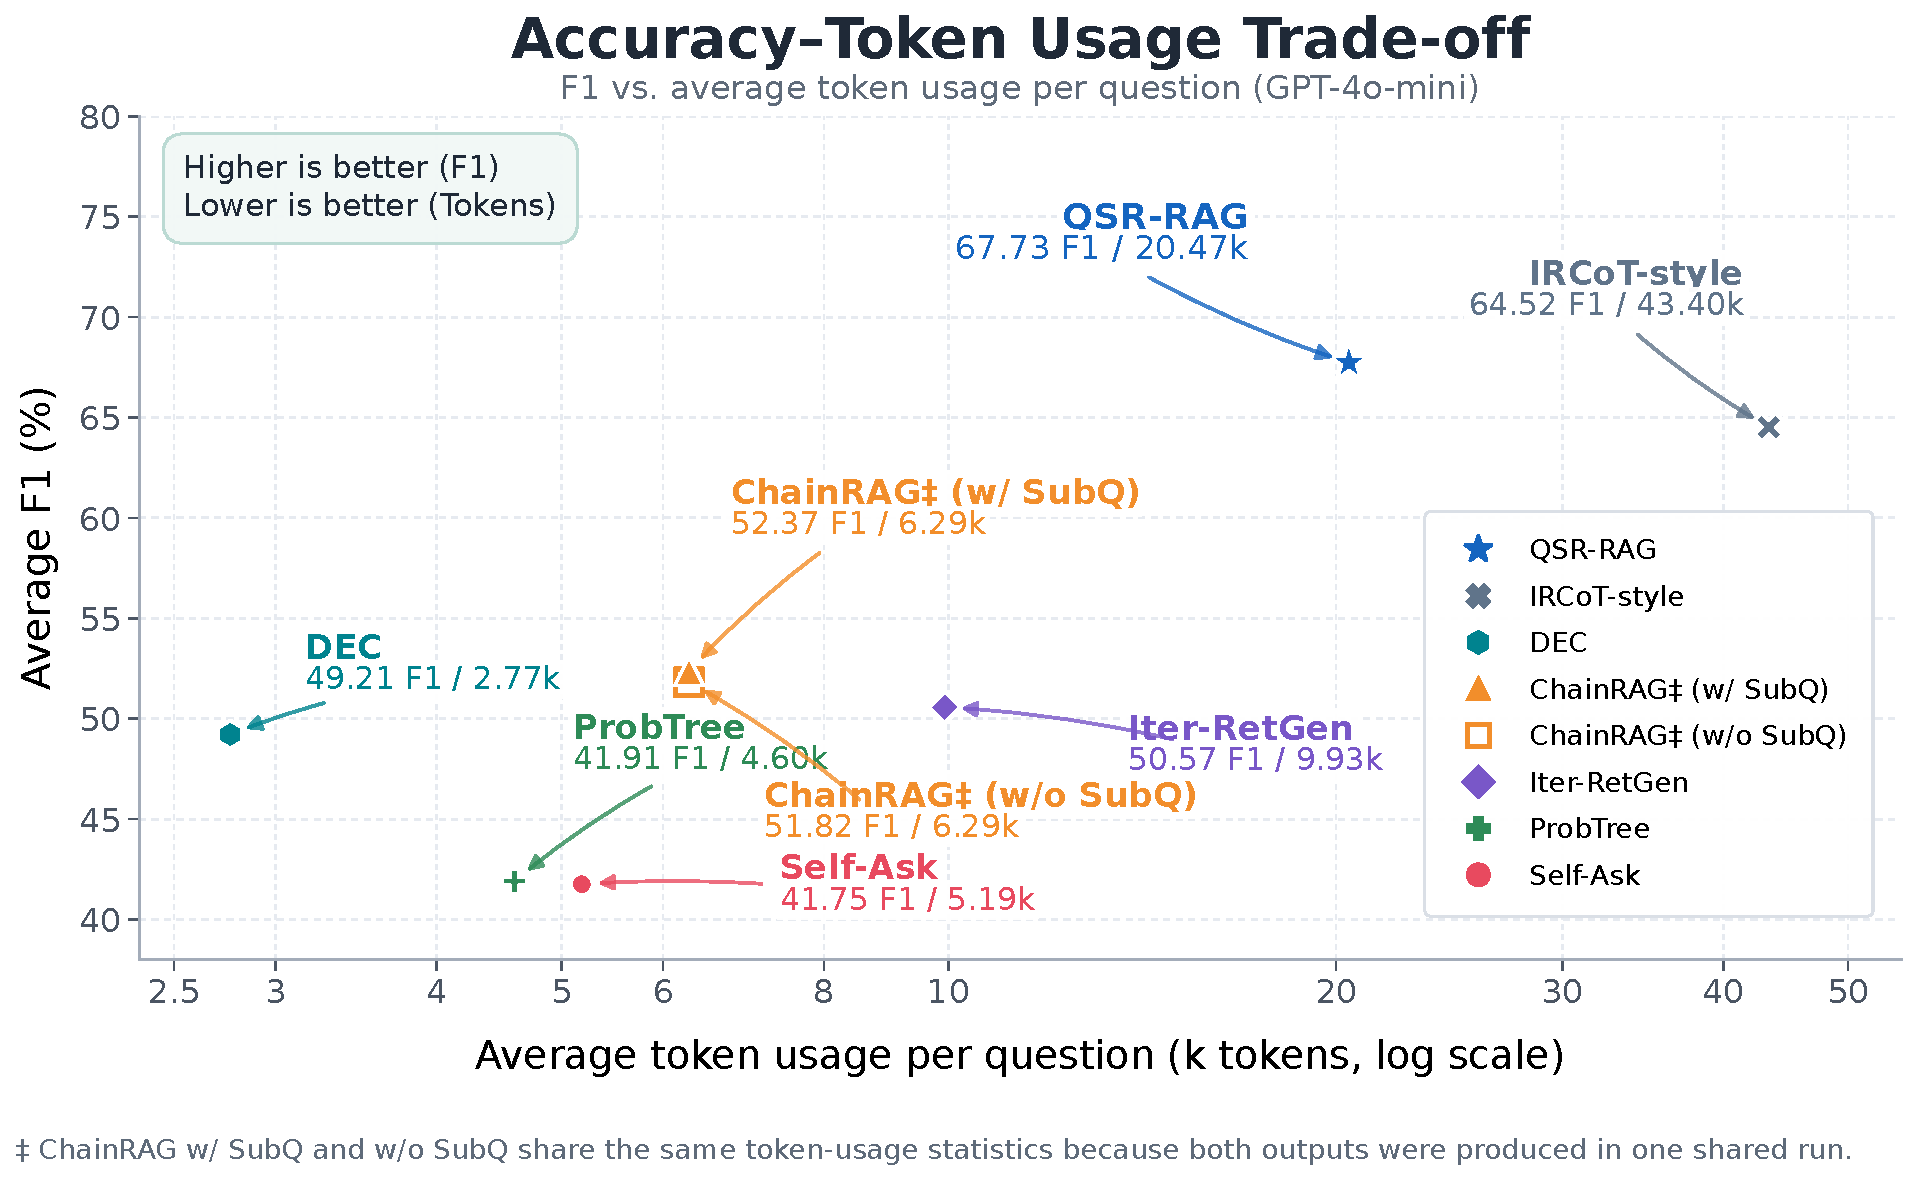
\includegraphics[width=\textwidth]{figures/figure3_accuracy_token.pdf}
		\caption{GPT-4o-mini 下三个数据集的平均 F1--Token 使用量权衡。横轴为每个问题所有 prompt 与 completion token 的总和（对数尺度），纵轴为三个数据集 F1 的算术平均。}
		\label{fig:token-tradeoff}
	\end{figure*}



	\subsection{跨方法 Token 使用量}

	\begin{table*}[t]
		\centering
		\caption{GPT-4o-mini 下各方法的 F1 与 Token 使用量（逐问题平均）。}
		\label{tab:token-usage}
		\small
		\setlength{\tabcolsep}{5pt}
		\begin{tabular}{lcccc}
			\toprule
			方法 & \makecell{HotpotQA\\F1 / Tokens (k)} & \makecell{2WikiMultiHopQA\\F1 / Tokens (k)} & \makecell{MuSiQue\\F1 / Tokens (k)} & 平均 Tokens (k)\\
			\midrule
			DEC                                           & 55.54 / 2.57  & 53.91 / 3.00  & 38.19 / 2.73  & 2.77\\
			Self-Ask\textsuperscript{\ddag}              & 53.82 / 4.37  & 35.77 / 5.82  & 35.67 / 5.37  & 5.19\\
			Iter-RetGen                                    & 50.22 / 8.38  & 55.17 / 9.77  & 46.32 / 11.64 & 9.93\\
			ProbTree                                       & 57.12 / 4.03  & 42.23 / 4.18  & 26.37 / 5.59  & 4.60\\
			IRCoT-style                                    & 70.47 / 34.12 & 72.08 / 48.31 & 51.02 / 47.75 & 43.40\\
			ChainRAG w/ SubQ\textsuperscript{\dag}        & 61.48 / 4.75  & 50.22 / 6.92  & 45.40 / 7.19  & 6.29\\
			ChainRAG w/o SubQ\textsuperscript{\dag}       & 65.06 / 4.75  & 48.72 / 6.92  & 41.67 / 7.19  & 6.29\\
			\textbf{QSR-RAG}                               & \textbf{73.65 / 21.23} & \textbf{74.19 / 19.58} & \textbf{55.35 / 20.61} & \textbf{20.47}\\
			\bottomrule
		\end{tabular}
	\end{table*}

	\noindent\textsuperscript{\dag} ChainRAG w/ SubQ 与 ChainRAG w/o SubQ 来自同一次共享运行，因此二者分别报告 F1，但共享 Token 使用量。\textsuperscript{\ddag} Self-Ask 在 MuSiQue 上的资源日志覆盖 498/500 个样本，因此其 token 统计只是近似值。由于缺少采用相同计量方式的完整 token 日志，Direct RAG 未列入该表。DEC 的 Token 使用量来自对应的 500 样本实验日志。


	\subsection{不同主干模型下 QSR-RAG 的详细资源使用}

	\begin{table*}[t]
		\centering
		\caption{QSR-RAG 在三个数据集和两个主干模型上的详细资源使用情况。Token 数量为逐问题平均值，单位为千（k）；Total LLM Calls 表示 500 个问题上的 LLM 总调用次数。}
		\label{tab:qsr-resource-detailed}
		\small
		\resizebox{\textwidth}{!}{%
			\begin{tabular}{llrrrrrrr}
				\toprule
				主干模型 & 数据集 & F1 & \makecell{平均 LLM\\调用 / 问题} & \makecell{LLM\\总调用} & \makecell{平均检索\\调用 / 问题} & \makecell{Prompt\\Tokens (k)} & \makecell{Completion\\Tokens (k)} & \makecell{总\\Tokens (k)}\\
				\midrule
				GPT-4o-mini & HotpotQA        & 73.65 & 12.02 & 6011 & 4.51 & 19.93 & 1.31 & 21.23\\
				GPT-4o-mini & 2WikiMultiHopQA & 74.19 & 10.81 & 5405 & 4.68 & 18.42 & 1.16 & 19.58\\
				GPT-4o-mini & MuSiQue         & 55.35 & 11.43 & 5716 & 4.36 & 19.46 & 1.15 & 20.61\\
				\midrule
				Qwen3-8B    & HotpotQA        & 72.25 & 10.02 & 5011 & 3.81 & 16.90 & 1.42 & 18.32\\
				Qwen3-8B    & 2WikiMultiHopQA & 71.88 & 10.04 & 5019 & 4.41 & 17.52 & 1.40 & 18.92\\
				Qwen3-8B    & MuSiQue         & 48.13 & 11.35 & 5676 & 4.29 & 19.51 & 1.55 & 21.06\\
				\bottomrule
		\end{tabular}}
	\end{table*}

	在表~\ref{tab:qsr-resource-detailed} 中，GPT-4o-mini 在三个数据集上的平均总 Token 使用量分别为 21.23k、19.58k 和 20.61k，每个问题平均 LLM 调用次数分别为 12.02、10.81 和 11.43。Qwen3-8B 分别使用 18.32k、18.92k 和 21.06k tokens，对应调用次数为 10.02、10.04 和 11.35。跨数据集取平均后，GPT-4o-mini 的 Token 使用量为 20.47k，Qwen3-8B 为 19.43k。



	\section{核心提示词与输出协议}
	\label{app:prompts}
	本节列出会影响已实现系统行为的核心提示词规则与输出格式；完整提示词可随代码一并发布。

	\subsection{问题生成器}
	问题生成器只决定每一轮下一条需要检索的局部信息；它既不直接回答最终问题，也不会预先生成完整推理链。它首先解析作为外层关系参数的、尚未解决的实体描述；当该实体变得明确后，再请求比较、布尔判断、排序、计数或选择问题所需的直接输入；如果都不适用，则询问最终的一跳信息需求。每条查询都从推理问题中出现的实体，或已经被已验证解答确认的实体出发，并且只跨越一个关系。同一轮不能返回两个存在依赖关系的局部问题；实现中每轮最多返回两个位于同一依赖层级、彼此独立的问题，格式如下：
	\begin{quote}\small
		\texttt{\{"questions": [\{"question": "... ?", "resolution\_target": "..."\}]\}}
	\end{quote}
	如果当前状态中已经没有新的未解决信息缺口，生成器返回 \texttt{\{"questions":[]\}}。三个数据集使用相同的核心规则和输出格式，只替换上下文演示样例；这些样例既不包含金标准答案，也不包含金标准支撑证据。

	\subsection{答案适配器}
	答案适配器判断检索到的支撑证据是否直接支持局部阅读器答案，并使其能够作为当前解答目标的取值。它检查的是关系，而不只是答案字符串是否出现在证据中。适配器保留局部阅读器给出的答案，只有当答案确实包含多个成员时才进行拆分，并返回 \texttt{evidence\_grounded} 和 \texttt{answer\_items}；它不会重新规划下一跳，也不会利用外部知识修复答案。

	\subsection{状态更新器}
	状态更新器只修改当前推理问题，而原始目标问题始终保持只读。更新必须保留最终信息需求、答案空间、尚未解析的外层关系、候选对象身份、比较方向以及逻辑操作；每个已验证解答只能应用于与其解答目标对齐的位置。替换操作把隐藏描述绑定到具体实体；增强操作则在直接替换可能破坏问题结构时，保留原问题并加入事实前提。如果安全检查判断某个候选更新无法保持这些约束，则当前问题保持不变。不过，由于该检查由模型驱动，它无法形式化保证每一次关系层面的语义漂移都能被检测出来。


	\section{定性推理轨迹}
	\label{app:cases}

	本节展示两个成功案例和一个失败案例，它们均来自本投稿中完整 QSR-RAG 的逐样本运行日志。案例选择的目标，是清晰展示\emph{推理问题 $\rightarrow$ 局部问题 $\rightarrow$ 已验证解答 $\rightarrow$ 状态更新 $\rightarrow$ 下一查询 / 最终答案}这一执行序列，同时避免使用问题语义与记录的金标准答案不一致的样例。除完整检索证据段落外，下文的问题、局部答案、更新输出和最终预测均直接来自运行日志。

	% ------------------------------------------------------------------
	% Breakable qualitative-trace helpers.
	% These commands expand to ordinary paragraphs / quote environments,
	% so LaTeX may naturally break across columns and pages.
	% ------------------------------------------------------------------
	\newcommand{\tracequestion}[2]{%
		\noindent\textbf{#1}\par
		\begin{quote}\small #2\end{quote}}
	\newcommand{\traceitem}[2]{%
		\noindent\textbf{#1} #2\par}
	\newcommand{\traceround}[1]{%
		\par\smallskip
		\noindent\rule{\columnwidth}{0.35pt}\par
		\noindent\textbf{第 #1 轮}\par\smallskip}
	\newcommand{\traceend}{%
		\par\smallskip\noindent\rule{\columnwidth}{0.55pt}\par\smallskip}

	\subsection{案例 1：增强操作保留比较候选项与答案空间}
	\label{case:hotpot-augmentation}

	\noindent\textbf{HotpotQA / \texttt{5a756b175542996c70cfaef7}.}
	该案例展示了一个并行比较过程：两个局部问题在同一依赖层级分别独立检索比较所需的数值。随后，更新器把两个数值都写回原始比较问题，但并不会把最终答案空间从“两座山峰”改变为“海拔数值本身”。

	\tracequestion{目标问题}{``Muztagh Ata 和 Manaslu，哪座山峰更高？''}

	\traceround{1}
	\tracequestion{推理问题}{``Muztagh Ata 和 Manaslu，哪座山峰更高？''}
	\tracequestion{生成的局部问题 1}{``Muztagh Ata 的海拔是多少？''}
	\traceitem{解答目标 1：}{Muztagh Ata 的海拔}
	\traceitem{已验证解答 1：}{\textbf{7509 米}}
	\tracequestion{生成的局部问题 2}{``Manaslu 的海拔是多少？''}
	\traceitem{解答目标 2：}{Manaslu 的海拔}
	\traceitem{已验证解答 2：}{\textbf{8163 米}}
	\traceitem{重写操作：}{\textbf{增强}（\texttt{CONTEXT\_INJECTION}）}
	\tracequestion{更新后的推理问题}{``Muztagh Ata 的海拔为 7509 米，Manaslu 的海拔为 8163 米。Muztagh Ata 和 Manaslu，哪座山峰更高？''}

	\traceround{2}
	\tracequestion{推理问题}{``Muztagh Ata 的海拔为 7509 米，Manaslu 的海拔为 8163 米。Muztagh Ata 和 Manaslu，哪座山峰更高？''}
	\traceitem{生成器输出：}{\texttt{NO\_NEW\_GAP}}
	\traceitem{状态更新：}{不再进行更新；控制权交给最终阅读器。}

	\traceend
	\traceitem{最终预测：}{\textbf{Manaslu}}
	\traceitem{金标准答案：}{\textbf{Manaslu}}

	这里，增强操作并不是为了生成一个新的数值比较查询，而是把两个已验证属性变成原始任务中的显式前提。下一轮生成器因此能够看到局部信息缺口已经被填补，同时目标问题仍然要求模型在 Muztagh Ata 和 Manaslu 之间进行选择。

	\subsection{案例 2：替换将隐藏描述转化为可直接检索的实体}
	\label{case:musique-substitution}

	\noindent\textbf{MuSiQue / \texttt{2hop\_\_590631\_110882}.}
	该示例首先把隐藏描述“作品的表演者”绑定到一个具体人物，然后询问该人物的出生日期。它还说明：当最终属性值已经以已验证解答的形式存在时，更新器并不一定需要强行把该值再次写回推理问题。

	\tracequestion{目标问题}{``《Unbreakable》的表演者出生于哪一天？''}

	\traceround{1}
	\tracequestion{推理问题}{``《Unbreakable》的表演者出生于哪一天？''}
	\tracequestion{生成的局部问题}{``谁表演了《Unbreakable》？''}
	\traceitem{解答目标：}{《Unbreakable》的表演者}
	\traceitem{局部答案 / 适配器：}{\textbf{James Cottriall} / \textbf{PASS}}
	\traceitem{重写操作：}{\textbf{替换}（\texttt{ENTITY\_BINDING}）}
	\tracequestion{更新后的推理问题}{``James Cottriall 的出生日期是什么？''}

	\traceround{2}
	\tracequestion{推理问题}{``James Cottriall 的出生日期是什么？''}
	\tracequestion{生成的局部问题}{``James Cottriall 出生于什么时候？''}
	\traceitem{解答目标：}{James Cottriall 的出生日期}
	\traceitem{局部答案 / 适配器：}{\textbf{1986 年 1 月 1 日} / \textbf{PASS}}
	\traceitem{候选状态更新：}{\texttt{CONTEXT\_INJECTION}}
	\traceitem{状态更新决策：}{\textbf{REJECTED / KEEP}；共享安全检查返回 \texttt{FINAL\_ANSWER\_SPACE\_LOST:attribute}，因此推理问题保持不变。}

	\traceround{3}
	\tracequestion{推理问题}{``James Cottriall 的出生日期是什么？''}
	\traceitem{生成器输出：}{\texttt{NO\_NEW\_GAP}}
	\traceitem{状态更新：}{不再进一步更新；最终阅读器直接使用已经验证的最终属性值。}

	\traceend
	\traceitem{最终预测：}{\textbf{1986 年 1 月 1 日}}
	\traceitem{金标准答案：}{\textbf{1986 年 1 月 1 日}}

	第 1 轮是一个直接的实体绑定替换：与解答目标对齐的隐藏描述“《Unbreakable》的表演者”被绑定到 James Cottriall，从而把下一跳转换为可以直接执行的一跳属性查询。第 2 轮已经获得目标日期。虽然候选重写被拒绝，但已验证解答记忆仍然保留 \textbf{1986 年 1 月 1 日}，随后生成器返回 \texttt{NO\_NEW\_GAP}。因此，QSR-RAG 并不要求每一轮都必须改变问题字符串；只有当重写通过安全检查时，它才会更新持久状态。

	\subsection{失败案例：状态重写与局部目标漂移可能绕过基于证据的准入}
	\label{case:musique-failure}

	\noindent\textbf{MuSiQue / \texttt{2hop\_\_555792\_30351}.}
	该问题与金标准答案在语义类型上是兼容的，因此可以从日志中逐步定位失败原因。到第 2 轮时，系统其实已经获得了正确最终答案 \textbf{Austrian government}。第一个错误发生在随后的状态写回中。更新器没有完整保留“在被 Ludwig von Mises 雇用时为……工作”这一条件性雇佣关系，而是生成了“奥地利政府雇用了 Hayek……Hayek 为谁工作？”此时状态已经发生语义漂移。基于这个状态，第 3 轮生成器进一步把原始的条件性解答目标扩大为“Hayek 的雇主”。答案适配器仍然可以为这个新的局部目标验证一个答案，却无法判断该目标本身已经不再与原始目标问题对齐。

	\tracequestion{目标问题}{``Hayek 在被《Omnipotent Government》的作者雇用时，为谁工作？''}

	\traceround{1}
	\tracequestion{推理问题}{``Hayek 在被《Omnipotent Government》的作者雇用时，为谁工作？''}
	\tracequestion{生成的局部问题}{``《Omnipotent Government》的作者是谁？''}
	\traceitem{解答目标：}{《Omnipotent Government》的作者}
	\traceitem{局部答案 / 适配器：}{\textbf{Ludwig von Mises} / \textbf{PASS}}
	\traceitem{重写操作：}{\textbf{替换}（\texttt{ENTITY\_BINDING}）}
	\tracequestion{更新后的推理问题}{``Hayek 在被 Ludwig von Mises 雇用时，为谁工作？''}

	\traceround{2}
	\tracequestion{推理问题}{``Hayek 在被 Ludwig von Mises 雇用时，为谁工作？''}
	\tracequestion{生成的局部问题}{``Hayek 在被 Ludwig von Mises 雇用时，为谁工作？''}
	\traceitem{解答目标：}{Hayek 在被 Ludwig von Mises 雇用时的雇主}
	\traceitem{局部答案 / 适配器：}{\textbf{Austrian government} / \textbf{PASS}}
	\traceitem{重要观察：}{此时，已验证解答实际上已经与金标准答案一致。}
	\tracequestion{更新后的推理问题}{``奥地利政府在 Hayek 被 Ludwig von Mises 雇用时雇用了 Hayek。Hayek 为谁工作？''}
	\traceitem{失败起点：}{状态写回已经无法完整保留原始条件性雇佣关系；在下一条局部问题生成之前，语义漂移就已经出现。}

	\traceround{3}
	\tracequestion{推理问题}{``奥地利政府在 Hayek 被 Ludwig von Mises 雇用时雇用了 Hayek。Hayek 为谁工作？''}
	\tracequestion{生成的局部问题}{``谁雇用了 Hayek？''}
	\traceitem{解答目标：}{Hayek 的雇主}
	\traceitem{局部答案 / 适配器：}{\textbf{Ludwig von Mises} / \textbf{PASS}}
	\traceitem{目标漂移：}{原来的条件性目标“Hayek 在被 Ludwig von Mises 雇用时的雇主”进一步被缩减为更宽泛的“Hayek 的雇主”。}
	\traceitem{重写决策：}{\textbf{KEEP}；候选更新不会改变当前推理问题。}

	\traceround{4}
	\traceitem{终止：}{生成器再次尝试生成已经解决的雇主目标，从而触发 \texttt{GENERATED\_RESOLVED\_TARGET}；随后控制权交给最终阅读器。}

	\traceend
	\traceitem{最终预测：}{\textbf{Ludwig von Mises}}
	\traceitem{金标准答案：}{\textbf{奥地利政府}}

	这个失败并不是因为系统没有找到正确证据：第 2 轮已经找到 \textbf{Austrian government}。更准确地说，错误连续发生在两个阶段。第一，状态更新器在写回正确解答时没有完整保留原始问题中的条件关系，从而在推理问题中造成关系层面的语义漂移。第二，生成器在这一漂移后的状态上继续生成了更宽泛的局部问题/解答目标。因此，第 3 轮适配器给出的 PASS 只表示 Ludwig von Mises 对\emph{新的局部目标}具有证据支持，并不能证明这个新目标仍然对应原始任务。该案例暴露出当前系统两个相互关联的局限：问题状态安全机制需要更强的“保持关系”状态转移验证；而基于证据的答案准入也需要配套的目标级验证，才能同时约束“这个答案是否有证据支持？”以及“我们现在验证的是否仍然是正确关系？”


\end{document}
